\documentclass[a4paper,10pt,twocolumn]{scrartcl} 

\usepackage{german}            
\usepackage[latin1]{inputenc}  
\usepackage{amsmath}           
\usepackage{amsfonts}          
\usepackage{amssymb}           
\usepackage{graphicx}         
\usepackage[T1]{fontenc}       
\usepackage{ae}              
\usepackage{typearea}	         
\usepackage{scrlayer-scrpage}         
\usepackage{lastpage}         
\usepackage[margin=10pt,font=small,labelfont=bf]{caption}
\renewcommand{\figurename}{Abb.}

\pagestyle{scrheadings}        
\typearea{16}                  
\renewcommand{\pnumfont}{%     
\normalfont\rmfamily\slshape}  


\begin{document}
\cfoot{\thepage /\pageref{LastPage}}     

\twocolumn[{\csname @twocolumnfalse\endcsname               
\titlehead{                                                  
	\begin{tabular*}{\textwidth}[]{@{\extracolsep{\fill}}lr}   
	Betreuer:  & \today\\                          
	\end{tabular*}                                             
	}
\title{Messung der Ausbreitungsgeschwindigkeit von elektromagnetischen Wellen in Koaxialkabeln und in der Luft} 
\author{J. Bergmeier und S. Steinicke}                    
\date{}                                                        
\maketitle                                                      
\vspace{-8ex}                                                   
\begin{abstract}                                                
ABSTRACT ABSTRACT ABSTRACT ABSTRACT ABSTRACT ABSTRACT ABSTRACT\\
\\ \\ 
\\ 
Versuchsdurchf�hrung: 10.09.2021\\       
Protokollabgabe:                
\\ 
\\ 
\end{abstract}
}]

\section{Einleitung}
Ein tiefes physikalisches Verst�ndnis der Elektromagnetischen Wellen ist heutzutage besonders wichtig, da technische Anwendungen von EM-Wellen im modernen Leben nicht mehr weg zu denken sind. Ein leicht zu untersuchendes Beispiel f�r den technischen Gebrauch von EM-Wellen ist das Koaxialkabel, welches z.B. bei der �bertragung in der Radartechnik oder der Musikproduktion Anwendung findet. Zum besseren Verst�ndnis des Koaxialkabels werden im folgenden Versuch Kerneigenschaften, wie der Wellenwiderstand, das Verhalten in Abh�ngigkeit des Verbrauchswiderstand, die D�mpfung des Kabels, dessen Dielektrizit�tskonstante, und die Ausbreitungsgeschwindigkeit im Kabel gemessen. Em-Wellen spielen auch im Medium Luft eine gro�e Rolle (W-Lan, LTE) und die dazugeh�rige Ausbreitungsgeschwindigkeit ist eine der wichtigsten Naturkonstanten, deshalb wollen wir diese separat messen.

\section{Theorie}
 Im Gro�teil der n�chsten Versuche spielen Koaxialkabel und elektromagnetische Wellen eine wichtige Rolle, weshalb wir zun�chst kurz deren wichtigsten Grundlagen nach \cite{a} und \cite{b} darstellen wollen. Das Kabel entspricht einem Hohlleiter mit einem Draht als Innenleiter und einer Ummantelung als Au�enleiter. Dazwischen befindet sich ein Dielektrikum in welchem die elektrischen Feldlinien radial nach au�en zeigen und das magnetische Feld in konzentrische Kreisen um den inneren Leiter gerichtet ist. Die Welle oder der Impuls breitet sich in endlicher Geschwindigkeit im Kabel aus und durch den ohmschen Widerstand der Leitungen und der endlichen Leitf�higkeit des Dielektrikums kommt es zur D�mpfung.  Da es sich bei dem Koaxialkabel um einen Zylinderkondensator handelt, lassen sich die Kerneigenschaften, wie D�mpfung \textit{D}, Ausbreitungsgeschwindigkeit \textit{v} und Wellenwiderstand \textit{Z}, aus der Induktivit�t \textit{L*} und Kapazit�t \textit{C*} pro L�ngeneinheit einfach berechnen:
\begin{align}
 D &= 20\log_{10} \frac{U(0)}{U(x)}dB\\
 v &= \frac{1}{\sqrt{L*C*}} &&= \frac{c}{\sqrt{\varepsilon_{r}\mu_{r}}}\\
 Z &= \sqrt{\frac{L*}{C*}} &&= \sqrt{\frac{\mu_{r}\mu_{0}}{\varepsilon_{r}\varepsilon_{0}}}\frac{1}{2\pi}\ln(\frac{d_{a}}{d_{i}})
\end{align}

Im folgenden wird f�r $\mu_{r}$ = 1 verwendet.\\
\\
In der technischen Anwendung ist es wichtig, dass es zu m�glichst keiner Reflexion am Verbraucherwiderstand, welcher am Koaxialkabel angeschlossen wurde,kommt. Dies dient der Sicherstellung der Signalintegrit�t. Dazu sollte der Verbraucherwiderstand an den Wellenwiederstand angepasst sein, wie man dem Reflexionskoeffizienten entnehmen kann:
\begin{align}
	\rho = \frac{R_{v}-Z}{R_{v}+Z} \label{Reflexionskoefizient}
\end{align}
Anhand der Gleichung \ref{Reflexionskoefizient} lassen sich drei ausgezeichnete F�lle ablesen. F�r $R_{v} \to \inf$ geht $\rho$ gegen eins und das hin- und zur�cklaufende Signal addieren sich, da die reflektiere Welle gleich der einlaufenden ist. Dies entspricht einem offenen Kabelende. F�r einen Kurzschluss ist $R_{v} \to 0$ und das reflektierte Signal l�uft invertiert, da $\rho = -1$ zur�ck, sodass sich beide Signale gegenseitig ausl�schen. Der letzte Fall wurde bereits erw�hnt. F�r $R_{v} = Z$ ist $\rho = 0$ und es kommt zu keiner Reflexion. Dieses Ph�nomen wird in den ersten Versuchsteilen untersucht. 
Zuletzt gehen wir noch kurz auf die Herausbildung stehender Wellen ein, da deren Verst�ndnis grundlegend f�r die Versuchsteile 3.4 und 3.5 ben�tigt wird. Stehende Wellen bilden sich immer dann, wenn sich eine hin- und zur�cklaufende aber ansonsten koh�rente Welle �berlagern. Dieses Ph�nomen kann gut am Koaxialkabel beobachtet werden, wenn an einem Ende Reflexion stattfindet. Die Wellen im Koaxialkabel sind ged�mpft und daher interferieren nicht zwei Wellen gleicher Amplituden, wodurch die Amplitude der stehenden Welle in den Knoten nicht komplett verschwindet. 

\section{Experiment}
\subsection{Messung des Wellenwiderstands eines Koaxialkabels}
\begin{figure}[htbp]
\begin{center}
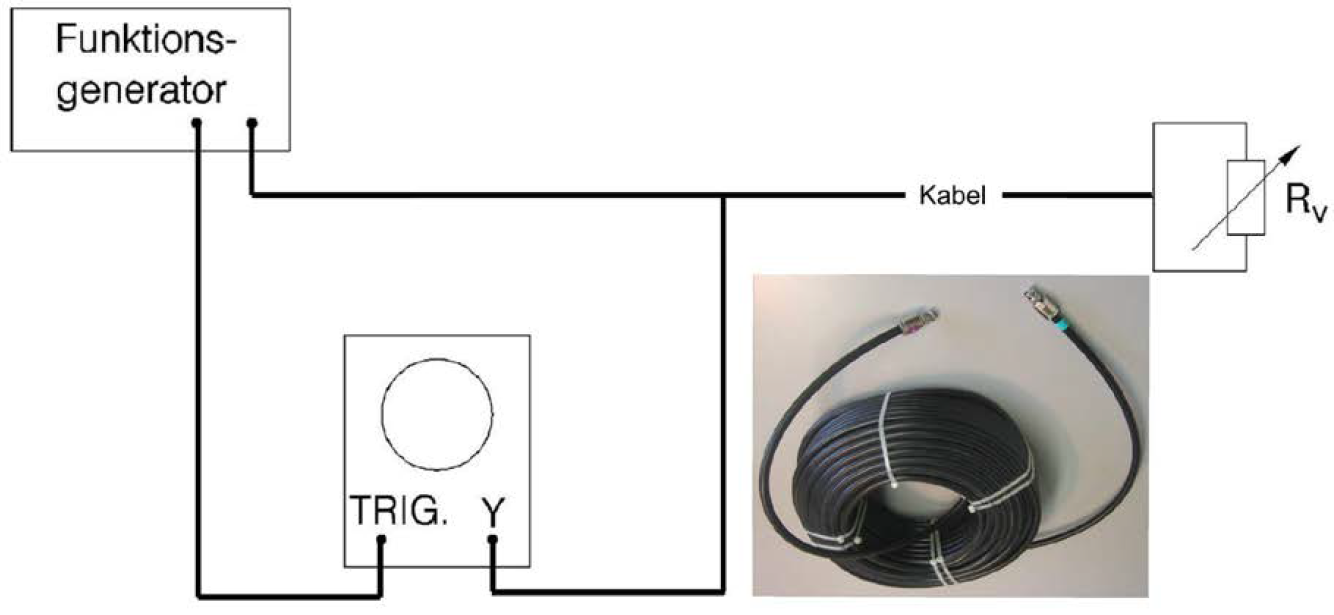
\includegraphics[width=0.9\linewidth]{Versuchsaufbau 3-1}
\caption[]{Versuchsaufbau 1: Der Funktionsgenerator gibt kurze Signale auf das Koaxialkabel, welches mit einem verstellbaren Verbraucherwiderstand abgeschlossen wird. Weiterhin ist ein Oszilloskop zur Beobachtung des Signals parallel dazu geschaltet. \cite{a}}
\label{Versuchsaufbau 3-1}
\end{center}
\end{figure}

\subsection{Messung mit verschiedenen Verbrauchswiderst�nden}
\begin{figure}[htbp]
	\begin{center}
		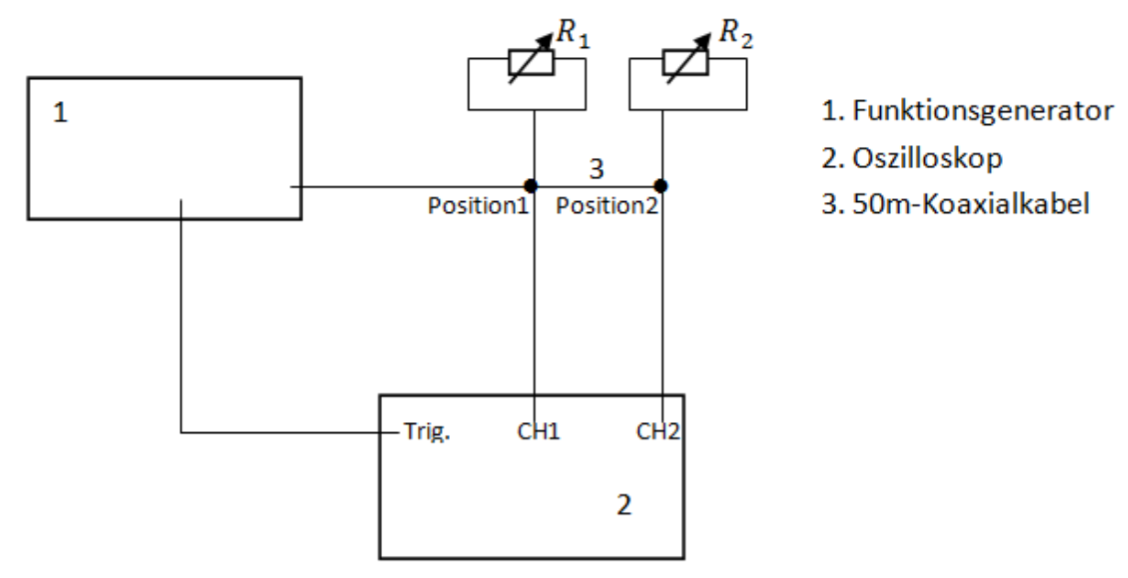
\includegraphics[width=0.9\linewidth]{Versuchsaufbau 3-2}
		\caption[]{Versuchsaufbau 2: Analoger Versuchsaufbau zur Abbildung \ref{Versuchsaufbau 3-1} mit einem weiteren generatorseitigen, verstellbaren Widerstand. Auf Channel 1 wird das generatorseitige Signal und auf Channel 2 das generatorferne Signal dargestellt.}
		\label{Versuchsaufbau 3-2}
	\end{center}
\end{figure}
\subsection{Messung der Ausbreitungsgeschwindigkeit in einem Koaxialkabel und einem Verz�gerungskabel}
\subsection{Darstellung von stehenden Wellen}
\subsection{Messung der Ausbreitungsgeschwindigkeit im Koaxialkabel mit Hilfe stehender Wellen}
\begin{figure}[htbp]
	\begin{center}
		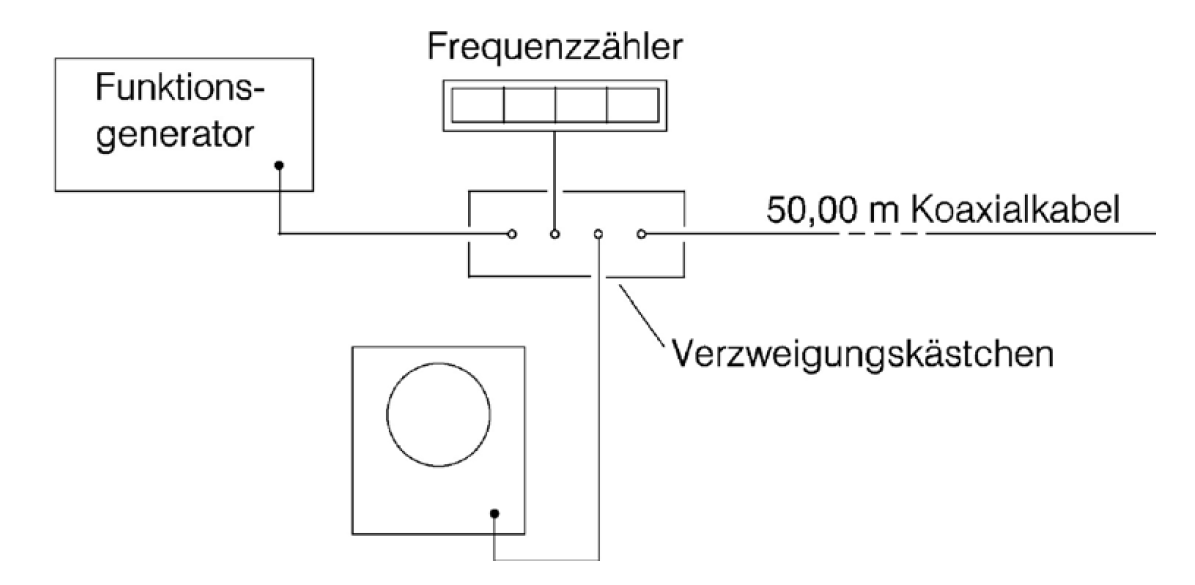
\includegraphics[width=0.9\linewidth]{Versuchsaufbau 3-5}
		\caption[]{Versuchsaufbau 3: �ber den Verteilungskasten werden die vom Funktionsgenerator erzeugten Signale vom Frequenzz�hler gemessen, auf das Koaxialkabel zur Ausbildung stehender Wellen �bertragen und vom Oszillograph visualisiert. \cite{a}}
		\label{Versuchsaufbau 3-5}
	\end{center}
\end{figure}

\subsection{Messung der Lichtgeschwindigkeit}
\begin{figure}[htbp]
	\begin{center}
		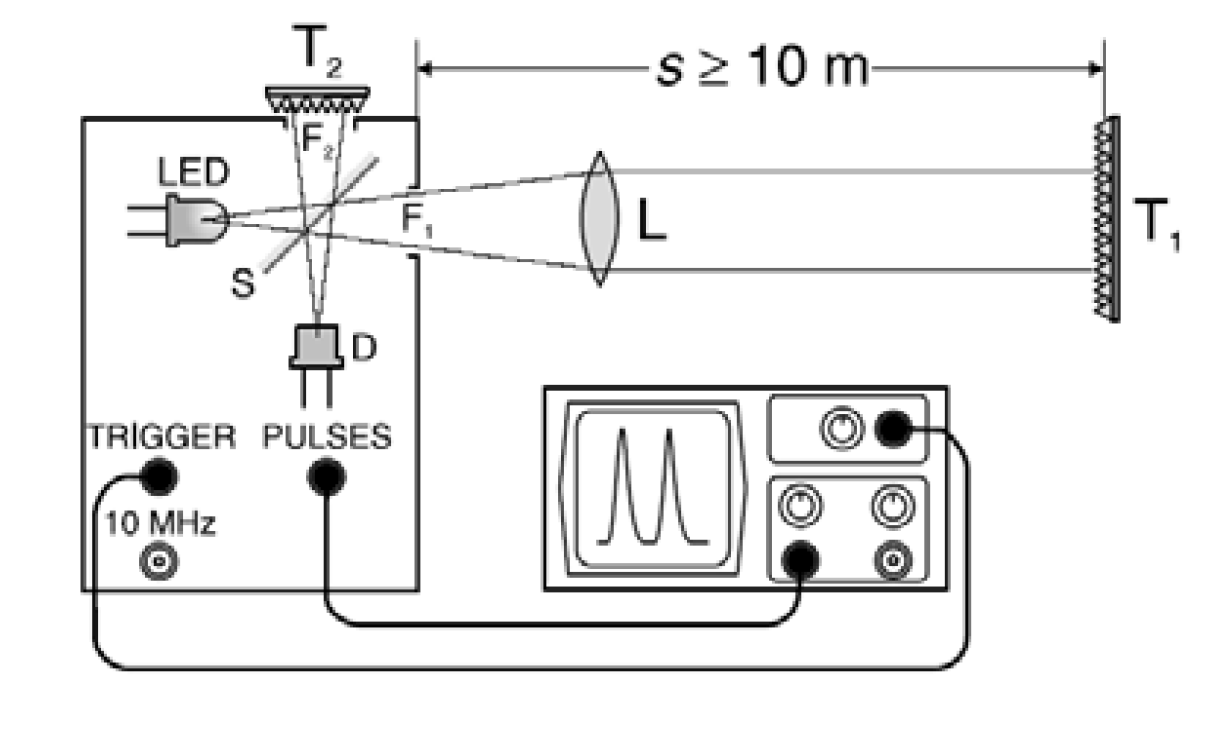
\includegraphics[width=0.9\linewidth]{Versuchsaufbau 3-6a}
		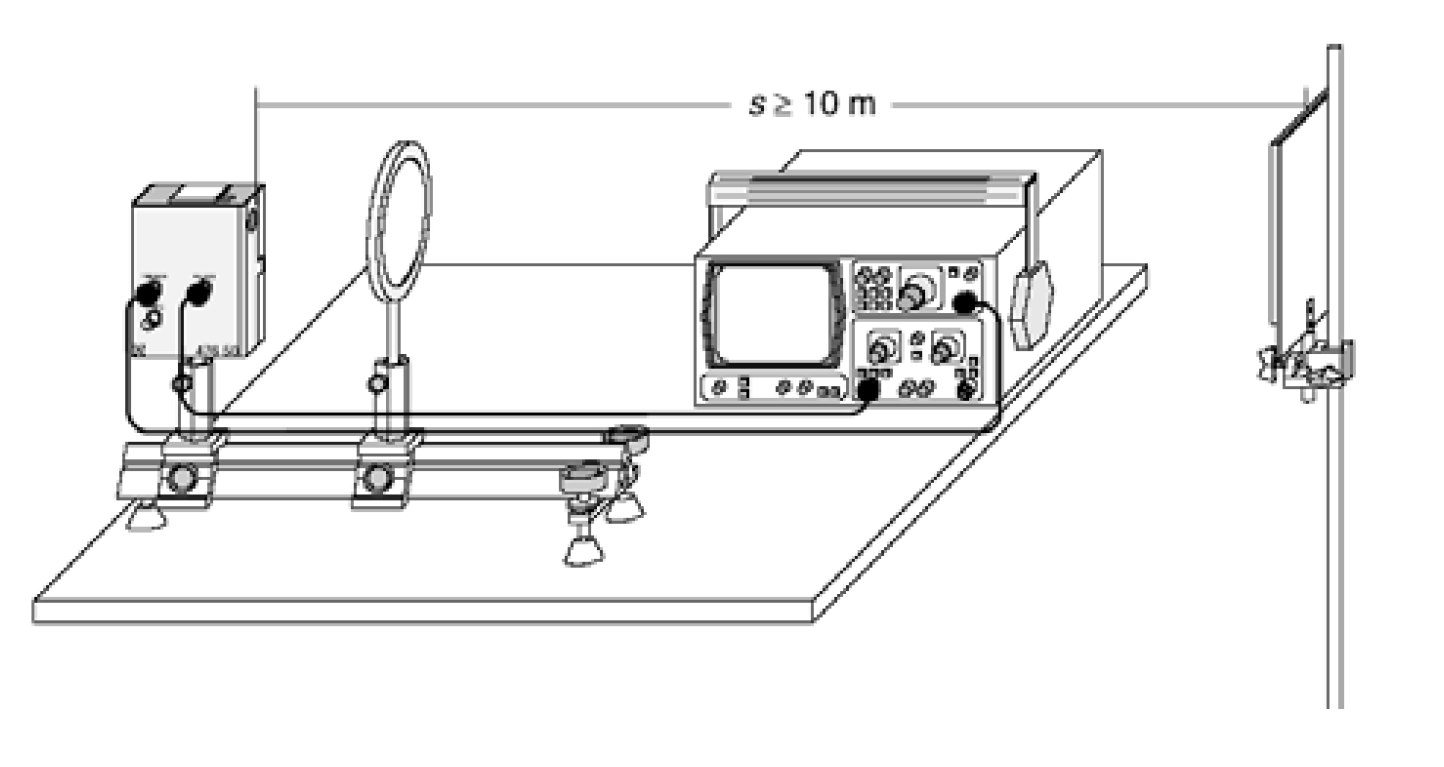
\includegraphics[width=0.9\linewidth]{Versuchsaufbau 3-6b}
		\caption[]{Versuchsaufbau 4:  aus einer LED werden kurze Lichtpulse durch eine Linse auf einen Tripelspiegel geschickt. Dessen Reflexion wird durch einen Strahlteiler auf einen Detektor geleitet. Der ausgegebene Spannungsverlauf wird mit dem Oszillograph verbildlicht. \cite{a} }
		\label{Versuchsaufbau 3-6}
	\end{center}
\end{figure}


\section{Zusammenfassung}


\begin{thebibliography}{}   
\bibitem{a} Physikalisches Grundpraktikum, Universit�t W�rzburg, Modul C1, Versuch 41, \glqq Messung der Ausbreitungsgeschwindigkeit von elektromagnetischen Wellen auf  Kabeln \grqq, 2021
\bibitem{b} Dieter Meschede, \glqq Gerthsen Physik\grqq, 25. Auflage, Springer Spektrum Berlin Heidelberg, 2015
\bibitem{c}
\end{thebibliography}

\section{Anhang}



\end{document}
